\documentclass[french]{extarticle}
\usepackage{rapport/lib/algorithmeUTF8}
\usepackage[utf8]{inputenc}
\usepackage[top=2.5cm, bottom=2.5cm, left=1.5cm, right=1.5cm]{geometry}
\usepackage{graphicx}
\usepackage[T1]{fontenc}
\usepackage[english]{babel}
\usepackage{fullpage}
\usepackage{color}
\usepackage[table]{xcolor}
\usepackage{listings}
\usepackage{moreverb}
\definecolor{darkWhite}{rgb}{0.94,0.94,0.94}
\lstset{
  aboveskip=3mm,
  belowskip=-2mm,
  backgroundcolor=\color{darkWhite},
  basicstyle=\footnotesize,
  breakatwhitespace=false,
  breaklines=true,
  captionpos=b,
  commentstyle=\color{red},
  deletekeywords={...},
  escapeinside={\%*}{*)},
  extendedchars=true,
  framexleftmargin=16pt,
  framextopmargin=3pt,
  framexbottommargin=6pt,
  frame=tb,
  inputencoding=utf8,
  keepspaces=true,
  keywordstyle=\color{blue},
  language=C,
  literate=
  {²}{{\textsuperscript{2}}}1
  {⁴}{{\textsuperscript{4}}}1
  {⁶}{{\textsuperscript{6}}}1
  {⁸}{{\textsuperscript{8}}}1
  {°}{{\textsuperscript{o}}}1
  {€}{{\euro{}}}1
  {ö}{{\"{o}}}1
  {ä}{{\"{a}}}1
  {ü}{{\"{u}}}1
  {é}{{\'{e}}}1
  {è}{{\`{e}}}1
  {ê}{{\^{e}}}1
  {ë}{{\¨{e}}}1
  {É}{{\'{E}}}1
  {Ê}{{\^{E}}}1
  {û}{{\^{u}}}1
  {ù}{{\`{u}}}1
  {â}{{\^{a}}}1
  {à}{{\`{a}}}1
  {á}{{\'{a}}}1
  {ã}{{\~{a}}}1
  {Á}{{\'{A}}}1
  {Â}{{\^{A}}}1
  {Ã}{{\~{A}}}1
  {ç}{{\c{c}}}1
  {Ç}{{\c{C}}}1
  {õ}{{\~{o}}}1
  {ó}{{\'{o}}}1
  {ô}{{\^{o}}}1
  {Õ}{{\~{O}}}1
  {Ó}{{\'{O}}}1
  {Ô}{{\^{O}}}1
  {î}{{\^{i}}}1
  {Î}{{\^{I}}}1
  {í}{{\'{i}}}1
  {Í}{{\~{Í}}}1,
  morekeywords={*,...},
  numbers=left,
  numbersep=10pt,
  numberstyle=\tiny\color{black},
  rulecolor=\color{black},
  showspaces=false,
  showstringspaces=false,
  showtabs=false,
  stepnumber=1,
  stringstyle=\color{gray},
  tabsize=4,
  title=\lstname,
}
\usepackage{newunicodechar}
\newunicodechar{fi}{fi}
\usepackage[unicode=true,pdfusetitle,bookmarks=true,bookmarksnumbered=false,bookmarksopen=false, breaklinks=false,pdfborder={0 0 0},pdfborderstyle={},backref=false,colorlinks=true]{hyperref}
\hypersetup{linkcolor=blue,urlcolor=blue}
\setcounter{tocdepth}{4}

\begin{document}
  \title{Département ASI / ITI de l'INSA Rouen \\
	Algorithmique et programmation avancée en C\\
	Rapport de Projet\\
	Projet Othello}
\author{MELO DA SILVA Alexis - MESBAH Zacharia\\
SAIVRES Jerôme - SI Ruixu}
\date{2019 - 2020}
\maketitle
\begin{figure}[h]
	\centering
	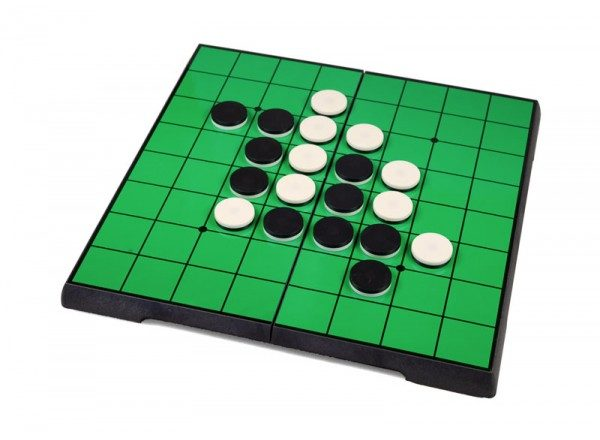
\includegraphics[width=12cm]{./sourcesIMAGES/othello.jpg}
\end{figure}

  \newpage
  \tableofcontents

  \newpage
  \section{Introduction}
    Dans le cadre du cours d'algorithmique et programattion avancée en C, notre promotion a travaillé, en groupes de4 à 5 personnes, à la réalisation d'un jeu d'Othello, entièrement développé en C. Nous avions pour cela l'aide de nos cours, des enseignants, et devions prendre l'initiative d'approfondir nos connaissances via les différents moyens à notre disposition (livres, internet), lorsque cela était nécessaire.

Nous avons réalisé ce jeu en équipe, et en suivant le cycle de développement en V, enseigné depuis la première année à l'INSA. Notre équipe est composée de 3 étudiants de STPI, un étudiant Euromed-SIC, et un étudiant intégré venant de DUT Info, tous les cinq suivant la formation ASI à l'INSA de Rouen Normandie. Avec nos approches différentes, et nos expériences plus ou moins importantes dans le domaine des projets informatiques, nous devions réussir à livrer dans les temps les dossiers et archives demandées.

  \newpage
  \section{Analyse du jeu de l'Othello}
    \subsection{Règle du jeu}
    \textbf{Plateau de jeu :}
    \begin{itemize}
        \item 64 cases (8x8)
        \item Colonne de a à h
        \item Ligne de 1 à 8 
        \item Initialiser avec deux pions noirs en e4 et d5 et deux pions blancs en d4 et e5
    \end{itemize}
    \textbf{Chaque joueur pose l'un après l'autre un pion de sa couleur}
    \begin{itemize}
        \item Obligation de capturer au moins un pion de l’adversaire
        \item Si un joueur ne peut pas capturer de pion : il passe son tour
    \end{itemize}
    \textbf{Capture de pions = retourner les pions adverses}
    \begin{itemize}
        \item Il faut placer ses pions à l'extrémité d'un alignement de pions adverses contigus terminé par un de ses propres pions (ex : B N N N N)
        \item Les alignements considérés peuvent être une colonne, une ligne, ou une diagonal
        \item Si le pion placé ferme plusieurs alignements, alors la capture des pions se fait sur tous les alignements
    \end{itemize}
    \textbf{Le jeu s'arrête quand les deux joueurs ne peuvent plus poser de pion}
    \begin{itemize}
        \item Aucun des deux joueurs ne peut jouer
        \item Le plateau ne comporte plus de case vide
    \end{itemize}
    \textbf{Score : nb de pions de sa couleur} \\ \\
    \textbf{Gagnant : le joueur ayant le score le plus grand}

\subsection{Différent mode de jeu}
    \textbf{Standard :}
    \begin{itemize}
        \item Joueur vs IA
        \item Choix de la couleur des pions que l’on donne à l’IA
    \end{itemize}
    \textbf{Tournoi :}
    \begin{itemize}
        \item Obligation de capturer au moins un pion de l’adversaire
        \item 10 secondes sur les machines des salles de TP pour jouer
        \item Communication à l’aide des entrées standards et des sorties standards du “broker”
    \end{itemize}

  \newpage
  \section{TADs}
    \documentclass[]{article}
\usepackage{babel}
\usepackage[utf8]{inputenc}
\usepackage{algorithmeUTF8} 
\begin{document}

	\begin{tad}
		\tadNom{Couleur}
		\tadDependances{Chaine de caractères}
		\begin{tadOperations}{Couleur}
			\tadOperation{Couleur}{\tadUnParam{Chaine de caractères}}{\tadUnParam{Couleur}}
			\tadOperation{CouleurOpposée}{\tadUnParam{Couleur}}{\tadUnParam{Couleur}}
			
		\end{tadOperations}
		\begin{tadAxiomes}
			\tadAxiome{CouleurOpposée( CouleurOpposée( Couleur ))) = Couleur}
		\end{tadAxiomes}
	\end{tad}
	
	\begin{tad}
		\tadNom{Pion}
		\tadDependances{Couleur}
		\begin{tadOperations}{Pion}
			\tadOperation{Pion}{\tadUnParam{Couleur}}{\tadUnParam{Pion}}
			\tadOperation{ObtenirCouleur}{\tadUnParam{Pion}}{\tadUnParam{Couleur}}
			\tadOperation{InverserCouleur}{\tadUnParam{Pion}}{\tadUnParam{Pion}}
		\end{tadOperations}
		\begin{tadAxiomes}
			\tadAxiome{InverserCouleur(InverserCouleur(Pion(Couleur))) = Pion}
		\end{tadAxiomes}
	\end{tad}
	
	\begin{tad}
		\tadNom{Position}
		\tadDependances{Colonne,Ligne}
		\begin{tadOperations}{Position}
			\tadOperation{Position}{\tadUnParam{Colonne x Ligne}}{\tadUnParam{Position}}
			\tadOperation{FixerColonne}{\tadUnParam{Colonne}}{\tadUnParam{Position}}
			\tadOperation{FixerLigne}{\tadUnParam{Ligne}}{\tadUnParam{Position}}
			\tadOperation{ObtenirColonne}{\tadUnParam{Position}}{\tadUnParam{Colonne}}
			\tadOperation{ObtenirLigne}{\tadUnParam{Position}}{\tadUnParam{Ligne}}
		\end{tadOperations}
		\begin{tadAxiomes}
		\end{tadAxiomes}
	\end{tad}
	
	\begin{tad}
		\tadNom{Coup}
		\tadDependances{Position,Pion,Plateau}
		\begin{tadOperations}{Coup}
			\tadOperation{Coup}{\tadUnParam{Position x Pion}}{\tadUnParam{Coup}}
			\tadOperation{ObtenirPosition}{\tadUnParam{Coup}}{\tadUnParam{Position}}
			\tadOperation{ObtenirPion}{\tadUnParam{Coup}}{\tadUnParam{Pion}}
			\tadOperation{EstValideCoup}{\tadUnParam{Plateau}}{\tadUnParam{Booleen}}
		\end{tadOperations}
		\begin{tadAxiomes}
		\end{tadAxiomes}
	\end{tad}
	
	\begin{tad}
		\tadNom{Plateau}
		\tadDependances{Position,Coup,Plateau,Pion}
		\begin{tadOperations}{Plateau}
			\tadOperation{Plateau}{\tadUnParam{Naturel x Naturel}}{\tadUnParam{Plateau}}
			\tadOperation{JouerCoup}{\tadUnParam{Plateau x Coup}}{\tadUnParam{Plateau}}
			\tadOperation{ObtenirPion}{\tadUnParam{Plateau x Position}}{\tadUnParam{Pion}}
			\tadOperation{CaseVide}{\tadUnParam{Plateau x Position}}{\tadUnParam{Booleen}}
			\tadOperation{Remplacer}{\tadUnParam{Plateau x Position}}{\tadUnParam{Plateau}}
		\end{tadOperations}
		\begin{tadAxiomes}
			\tadAxiome{ObtenirPion(JouerCoup(Plateau,Coup(Position,Pion)), Position) = Pion}
			\tadAxiome{Remplacer(Remplacer(Plateau,Position),Position) = Plateau}
		\end{tadAxiomes}
	\end{tad}
	
	\begin{tad}
		\tadNom{Coups}
		\begin{tadOperations}{Coups}
			\tadOperation{Coups}{}{\tadUnParam{Ensemble<Coup>}}
			\tadOperation{AjouterCoup}{\tadUnParam{Coups x Coup}}{\tadUnParam{Coups}}
			\tadOperation{RetirerCoup}{\tadUnParam{Coups x Coup}}{\tadUnParam{Coups}}
			\tadOperation{NombreCoups}{\tadUnParam{Coups}}{\tadUnParam{Naturel}}
		\end{tadOperations}
		
	\end{tad}
	
\end{document}

  \newpage
  \section{Analyse descendante}
    \begin{figure}[h]
  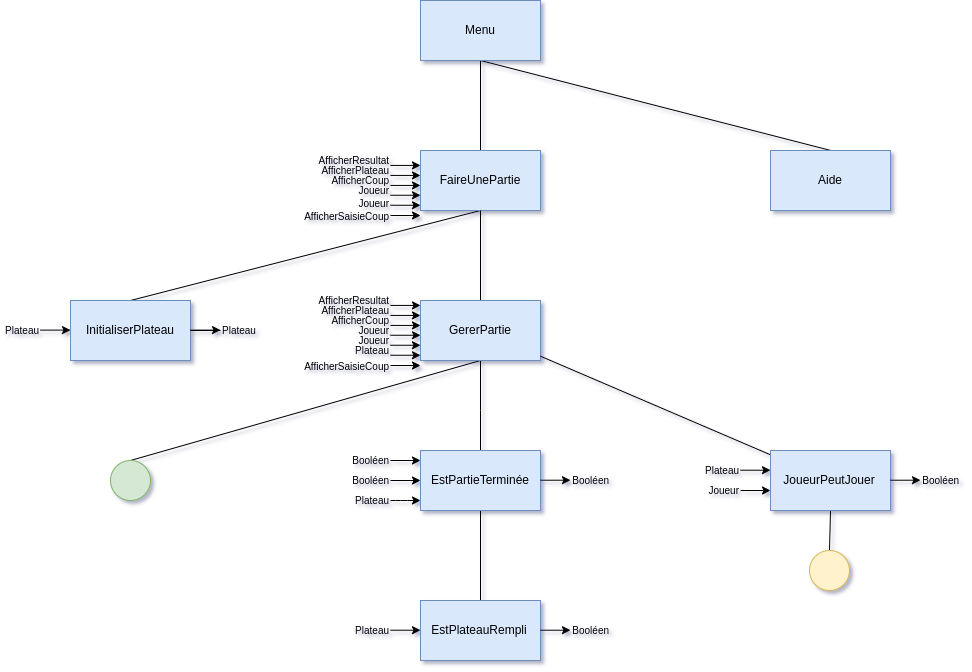
\includegraphics[width=18cm]{./sourcesIMAGES/analyse_main.png}
  \caption{Base principale de l'analyse descendante}
\end{figure}
\newpage
\begin{figure}[h]
  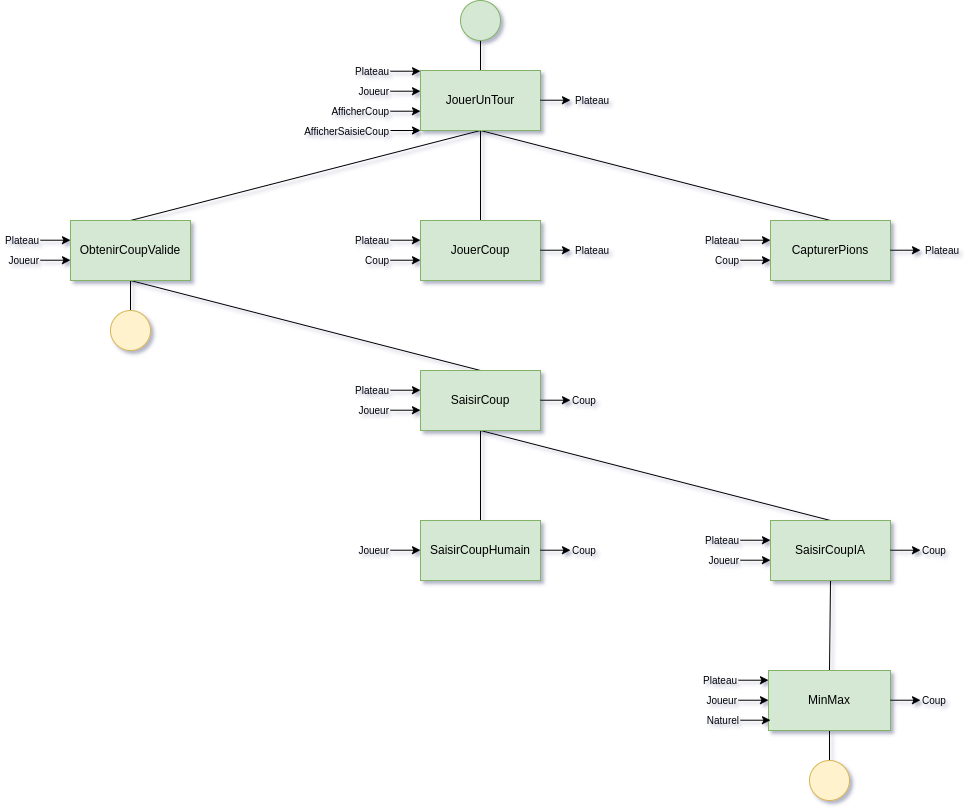
\includegraphics[width=18cm]{./sourcesIMAGES/analyse_jouerUnTour.png}
  \caption{Sous arbre de l'analyse descendante découlant de la méthode JouerUnTour}
\end{figure}
\begin{figure}[h]
  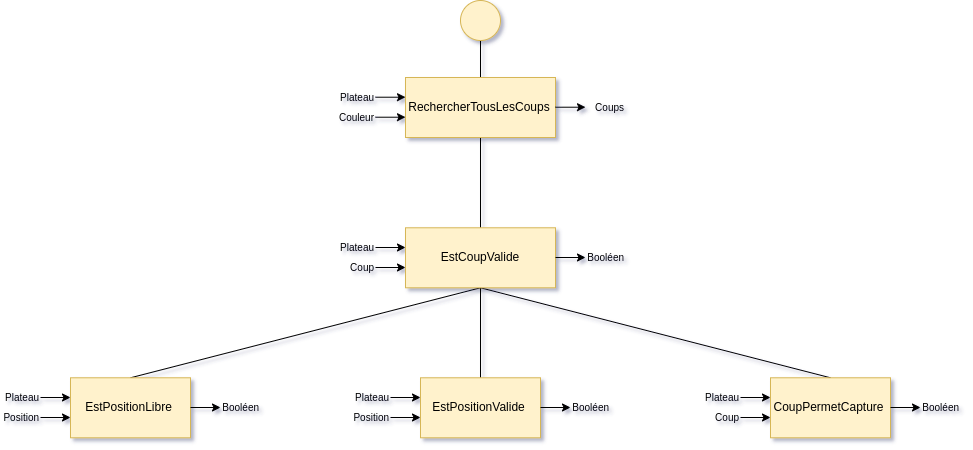
\includegraphics[width=18cm]{./sourcesIMAGES/analyse_chercherTousLesCoups.png}
  \caption{Sous arbre de l'analyse descendante découlant de la méthode RechercherTousLesCoups}
\end{figure}


  \newpage
  \section{Conception preliminaire}
       \subsection{TAD Couleur}
    \begin{algorithme}
    \signaturefonction{creerBlanc}{}{\textbf{Couleur}}
    \signaturefonction{creerNoir}{}{\textbf{Couleur}}
    \signaturefonction{creerNeutre}{}{\textbf{Couleur}}
    \signaturefonction{ObtenirCouleurOpposee}{couleur : Couleur}{\textbf{Couleur}}
    \signaturefonction{estNeutre}{}{\textbf{Couleur}}
    \signaturefonction{FixerCouleurOpposee}{couleur : Couleur, couleurOpposee : Couleur}{\textbf{Couleur}}
    \end{algorithme}
    \subsection{TAD Direction}
     \begin{algorithme}
    \signaturefonction{creerH}{}{\textbf{Direction}}
    \signaturefonction{creerHD}{}{\textbf{Direction}}
    \signaturefonction{creerD}{}{\textbf{Direction}}
    \signaturefonction{creerBD}{}{\textbf{Direction}}
    \signaturefonction{creerB}{}{\textbf{Direction}}
    \signaturefonction{creerBG}{}{\textbf{Direction}}
    \signaturefonction{creerG}{}{\textbf{Direction}}
    \signaturefonction{creerHG}{}{\textbf{Direction}}
    \signaturefonction{ObtenirDecalageColonne}{direction : Direction}{\textbf{-1},\textbf{0},\textbf{1}}
    \signaturefonction{ObtenirDecalageLigne}{direction : Direction}{\textbf{-1},\textbf{0},\textbf{1}}
    \end{algorithme}
    \subsection{TAD Etat}
     \begin{algorithme}
    \signaturefonction{creerTermine}{}{\textbf{Etat}}
    \signaturefonction{creerEnCours}{}{\textbf{Etat}}
    \signaturefonction{creerBloque}{}{\textbf{Etat}}
    \signaturefonction{EtatDeLaPartie}{plateauDeJeu : PLateau, joueurActuel : Couleur}{\textbf{Etat}}
    \end{algorithme}
    
    
    \subsection{TAD Position}
\begin{algorithme}
	\signaturefonction{CreerPosition}{c : Colonne, l : Ligne}{Position}
	\signatureprocedure{AppliquerDirection}{\paramEntreeSortie unePostion : Position, \paramEntree uneDirection : Direction}
	\signaturefonction{FixerColonne}{c : Colonne, l : Ligne}{Position}
	\signaturefonction{FixerLigne}{c : Colonne}{Position}
	\signaturefonction{ObtenirColonne}{unePostion : Position}{Colonne}
	\signaturefonction{ObtenirLigne}{unePostion : Position}{Ligne}
	\signaturefonction{EstEgalPosition}{position1, position2 : Position}{\booleen}
\end{algorithme}


\subsection{TAD Coup}
\begin{algorithme}
	\signaturefonction{CreerCoup}{unePostion : Position, uneCouleur : Couleur}{Coup}
	\signaturefonction{ObtenirPosition}{unCoup : Coup}{Position}
	\signaturefonction{ObtenirCouleur}{unCoup : Coup}{Couleur}
	\signaturefonction{EstCoupValide}{unPlateau : Plateau}{\booleen}
	\signaturefonction{EstEgalCoup}{coup1, coup2 : Coup}{\booleen}
\end{algorithme}


\subsection{TAD Coups}
\begin{algorithme}
	\signaturefonction{CreerCoups}{}{Ensemble $<$Coup$>$} \\
	Nous prendrons pour la suite :  Coups = Ensemble $<$Coup$>$
	\signaturefonction{EstVide}{lesCoups : Coups}{\booleen}
	\signatureprocedure{AjouterCoup}{\paramEntreeSortie lesCoups : Coups, \paramEntree unCoup : Coup}
	\signatureprocedure{RetirerCoup}{\paramEntreeSortie lesCoups : Coups, \paramEntree unCoup : Coup}
	\signaturefonction{ObtenirCoup}{lesCoups : Coups}{Coup}
	\signaturefonction{ObtenirNombreDeCoups}{lesCoups : Coups}{\naturel}
	\signaturefonction{EstPresent}{lesCoups : Coups, unCoup : Coup}{\booleen}
\end{algorithme}


\subsection{TAD Plateau}
\begin{algorithme}
	\signaturefonction{CreerPlateau}{}{Plateau}
	\signatureprocedure{InitialiserPlateau}{\paramEntreeSortie unPlateau : Plateau}
	\signatureprocedure{JouerCoup}{\paramEntreeSortie unPlateau : Plateau, \paramEntree unCoup : Coup}
	\signaturefonction{ObtenirCouleurAvecPosition}{unPlateau : Plateau, unePosition : Position}{Couleur}
	\signaturefonction{EstPositionLibre}{unPlateau : Plateau, unePosition : Position}{\booleen}
	\signaturefonction{ObtenirTaille}{unPlateau : Plateau}{\naturel}
	\signaturefonction{EstRempli}{unPlateau : Plateau}{\booleen}
	\signaturefonction{CalculerPoints}{unPlateau : Plateau, uneCouleur : Couleur}{\naturel}
	\signaturefonction{EstPositionValide}{unPlateau : Plateau, unePosition : Position}{\booleen}
	\signatureprocedure{CapturerPions}{\paramEntreeSortie unPlateau : Plateau, \paramEntree unCoup : Coup}
	\signatureprocedure{CapturerPionsDansDirections}{\paramEntreeSortie unPlateau : Plateau, \paramEntree unCoup : Coup, \paramEntree uneDirection : Direction}
\end{algorithme}


\subsection{TAD Ligne}
\begin{algorithme}
	\signaturefonction{ObtenirLigneDepuisInt}{ligNum : 1 .. Taille}{Ligne}
	\signaturefonction{ObtenirNumeroLigne}{l : Ligne}{1 .. Taille}
	\signaturefonction{EstEgalLigne}{l1, l2 : Ligne}{\booleen}
\end{algorithme}


\subsection{TAD Colonne}
\begin{algorithme}
	\signaturefonction{ObtenirColonneDepuisInt}{colNum : 1 .. Taille}{Colonne}
	\signaturefonction{ObtenirColonneDepuisInt}{colChar : Char}{Colonne}
	\signaturefonction{ObtenirNumeroColonne}{c : Colonne}{1 .. Taille}
	\signaturefonction{EstEgalColonne}{c1, c2 : Colonne}{\booleen}
\end{algorithme}

    \subsection{Analyse descendante bleue}	
	\begin{algorithme}
		\signaturefonction{FaireUnePartie}{AfficherResultat, AfficherPlateau, AfficherCoup, AfficherSaisieCoup : Fonction, j1, j2 : Joueur}{}
	\end{algorithme}
	\begin{algorithme}
		\signatureprocedure{InitialiserPlateau}{\paramEntreeSortie plateau : Plateau}
	\end{algorithme}
	\begin{algorithme}
		\signatureprocedure{GererPartie}{\paramEntree AfficherResultat, \paramEntree AfficherPlateau, \paramEntree AfficherCoup, \paramEntree AfficherSaisieCoup : Fonction, \paramEntree j1, \paramEntree j2 : Joueur, \paramEntreeSortie plateau : Plateau}
	\end{algorithme}
	\begin{algorithme}
		\signaturefonction{EstPartieTerminee}{plateau : Plateau, j1PeutJouer, j2PeutJouer : \booleen}{\booleen}
	\end{algorithme}
	\begin{algorithme}
		\signaturefonction{JoueurPeutJouer}{plateau : Plateau, joueur : Joueur}{\booleen}
	\end{algorithme}
	\begin{algorithme}
		\signaturefonction{EstRempli}{plateau : Plateau}{\booleen}
	\end{algorithme}
	
\subsection{Analyse descendante verte}	
	\begin{algorithme}
		\signatureprocedure{JouerUnTour}{\paramEntreeSortie plateau : Plateau, \paramEntree joueur : Joueur, \paramEntree AfficherCoup, \paramEntree AfficherSaisieCoup : Fonction}
	\end{algorithme}
	\begin{algorithme}
		\signatureprocedure{CapturerPions}{\paramEntreeSortie plateau : Plateau, \paramEntree coup : Coup}
	\end{algorithme}
	\begin{algorithme}
		\signatureprocedure{JouerCoup}{\paramEntreeSortie plateau : Plateau, \paramEntree coup : Coup}
	\end{algorithme}
	\begin{algorithme}
		\signaturefonction{ObtenirCoupValide}{plateau : Plateau, joueur : Joueur}{\textbf{Coup}}
	\end{algorithme}
	\begin{algorithme}
		\signaturefonction{SaisirCoup}{j : Joueur, plateau : Plateau}{\textbf{Coup}}
	\end{algorithme}
	\begin{algorithme}
		\signaturefonction{SaisirCoupHumain}{j : Joueur}{\textbf{Coup}}
	\end{algorithme}
	\begin{algorithme}
		\signaturefonction{SaisirCoupIA}{j : Joueur, plateau : Plateau}{\textbf{Coup}}
	\end{algorithme}
	\begin{algorithme}
		\signaturefonction{MinMax}{plateau : Plateau, joueurAMaximiser : Joueur, profondeur : \naturel}{\textbf{Coup}}
	\end{algorithme}

\subsection{Analyse descendante jaune}	
	\begin{algorithme}
		\signaturefonction{RechercherTousLesCoups}{plateauDeJeu : Plateau, couleurJoueurActuel : Couleur}{\textbf{Coups}}
	\end{algorithme}
	\begin{algorithme}
		\signaturefonction{EstCoupValide}{plateau : Plateau, coup : Coup}{\textbf{\booleen}}
	\end{algorithme}
	\begin{algorithme}
		\signaturefonction{EstPositionLibre}{plateau : Plateau, position : Position}{\textbf{\booleen}}
	\end{algorithme}
	\begin{algorithme}
		\signaturefonction{EstPositionValide}{plateau : Plateau, position : Position}{\textbf{\booleen}}
	\end{algorithme}
	\begin{algorithme}
		\signaturefonction{CoupPossibleDansUneDirectionQuelconque}{plateau : Plateau, coup : Coup}{\textbf{\booleen}}
	\end{algorithme}
	\begin{algorithme}
		\signaturefonction{CoupPossibleDansDirection}{plateau : Plateau, coup : Coup, direction : Direction}{\textbf{\booleen}}
	\end{algorithme}

  \newpage
  \section{Types}
    \begin{algorithme}

	\begin{enregistrement}{Couleur}
		\champEnregistrement{nom}{Chaine de caractères}
		\champEnregistrement{hexa}{Chaine de caractères}
		\champEnregistrement{couleurOpposee}{Couleur}
		\champEnregistrement{symbole}{Caractère}
		\champEnregistrement{estNeutre}{\booleen}
	\end{enregistrement}
\\
	\begin{enregistrement}{Pion [DEPRECATED]}
		\champEnregistrement{couleur}{Couleur}
	\end{enregistrement}
\\
	\begin{enregistrement}{Position}
		\champEnregistrement{ligne}{Ligne}
		\champEnregistrement{colonne}{Colonne}
	\end{enregistrement}
\\

	\begin{enregistrement}{Coup}
		\champEnregistrement{couleur}{Couleur}
		\champEnregistrement{position}{Position}
	\end{enregistrement}
\\\\
	\textbf{Type} Plateau \textbf{=} Tableau[1...Taille][1...Taille] de Couleur
\\\\
	\textbf{Type} Coups \textbf{=} Ensemble$<$Coup$>$
\\\\
	\textbf{Type} Ligne \textbf{=} 1...Taille
\\\\
	\textbf{Type} Colonne \textbf{=} 1...Taille
\\\\
	\begin{enregistrement}{Direction}
		\champEnregistrement{decalageLigne}{\{-1,0,1\}}
		\champEnregistrement{decalageColonne}{\{-1,0,1\}}
	\end{enregistrement}
\\\\
	\textbf{Type} Etat \textbf{=} {\{EN COURS, BLOQUE, TERMINE\}}


\end{algorithme}


  \newpage
  \section{Conception détaillée}
    \begin{algorithme}
	\small
	\procedure
	{Initialiser Plateau}
	{\paramEntreeSortie p : Plateau}
	{ObtenirTaille(p) : \naturelNonNul \\
	blanc, noir, neutre : Couleur}
	{
	\affecter{neutre}{creerNeutre()}
	\affecter{blanc}{creerBlanc()}
	\affecter{noir}{creerNoir()}
	\pour{i}{1}{ObtenirTaille(p)}{}{

		\pour{j}{1}{ObtenirTaille(p)}{}{

			\instruction{JouerCoup(plateau,Coup(neutre,Position(Ligne(i),Colonne(j))))}
		}
	}

	\instruction{JouerCoup(plateau,Coup(blanc,Position(Ligne(ObtenirTaille(p) div 2),Colonne(ObtenirTaille(p) div 2))))}

	\instruction{JouerCoup(plateau,Coup(blanc,Position(Ligne(ObtenirTaille(p) div 2 + 1),Colonne(ObtenirTaille(p) div 2 + 1))))}

	\instruction{JouerCoup(plateau,Coup(noir,Position(Ligne(ObtenirTaille(p) div 2),Colonne(ObtenirTaille(p) div 2 + 1))))}

	\instruction{JouerCoup(plateau,Coup(noir,Position(Ligne(ObtenirTaille(p) div 2 + 1),Colonne(ObtenirTaille(p) div 2))))}
	}
\end{algorithme}

    \begin{algorithme}
	\small
	\fonction
	{FaireUnePartie}
	{joueur = Couleur, ProfondeurIA = Naturel}
	{}
	{plateau = Plateau}
	{
	\affecter{plateau}{InitialiserPlateau()}
	\tantque{non FinirLaPartie}{
		\affecter{plateau}{JouerUnTour(plateau, joueur, ProfondeurIA)}
		\affecter{joueur}{Inverser(joueur)}
	}
	}
\end{algorithme}
    \begin{algorithme}
	\small
	\procedure
	{GererPartie}
	{\paramEntree AfficherResultat, \paramEntree AfficherPlateau, \paramEntree AfficherCoup : Fonction, \paramEntree j1, \paramEntree j2 : Joueur, \paramEntreeSortie plateau : Plateau}
    {j1PeutJouer, j2PeutJouer, partieTerminee : \booleen \\
    important : ChaineDeCaractères \\
    premierJoueur, secondJoueur : Joueur
    }
	{
    \affecter{j1PeutJouer}{Vrai}
    \affecter{j2PeutJouer}{Vrai}
    \affecter{partieTerminee}{Faux}
    \instruction{SetOrdreJoueurs(premierJoueur, secondJoueur, j1, j2)}
    \instruction{AfficherPlateau(plateau)}
    \tantque{non partieTerminee}{
        \affecter{j1PeutJouer}{JoueurPeutJouer(plateau, premierJoueur)}
		\sialorssinon {j1PeutJouer}{
            \instruction{JouerUnTour(plateau,premierJoueur, AfficherCoup)}
            \instruction{AfficherPlateau(plateau)}
            \affecter{partieTerminee}{EstPartieTerminee(plateau, j1PeutJouer, j2PeutJouer)}
        }
            {
            {\sialorssinon{EstIA(premierJoueur)}{
                \instruction{ecrire("passe$\backslash$n")}
            }
                {
                \instruction{lire(important)}
                }
            }
        }
        \affecter{j2PeutJouer}{JoueurPeutJouer(plateau, secondJoueur)}
		\sialorssinon {j1PeutJouer}{
            \instruction{JouerUnTour(plateau,secondJoueur, AfficherCoup)}
            \instruction{AfficherPlateau(plateau)}
        }
            {
            {\sialorssinon{EstIA(secondJoueur)}{
                \instruction{ecrire("passe$\backslash$n")}
            }
                {
                \instruction{lire(important)}
                }
            }
        }
        \affecter{partieTerminee}{EstPartieTerminee(plateau, j1PeutJouer, j2PeutJouer)}
    }
    \instruction{AfficherResultat(plateau,j1,j2)}
	}
\end{algorithme}
    \begin{algorithme}
	\small
	\procedure
	{JouerUnTour}
	{\paramEntreeSortie plateau : Plateau, \paramEntree joueur : Joueur, \paramEntree AfficherCoup, \paramEntree AfficherSaisieCoup : Fonction}
	{coupAJouer : Coup}
	{
	\instruction{AfficherSaisieCoup(joueur)}
	\affecter{coupAJouer}{ObtenirCoupValide(plateau, joueur)}
	\instruction{JouerCoup(plateau, coupAJouer)}
	\instruction{CapturerPions(plateau, coupAJouer)}
	\sialors{EstIA(joueur)}
		{\instruction{AfficherCoup(coupAJouer)}}
	}
\end{algorithme}
    \begin{algorithme}
	\small
	\fonction
	{EstPartieTerminee}
	{plateau : Plateau, j1PeutJouer, j2PeutJouer : \booleen}
	{\booleen}
    {}
    {
    \sialorssinon {(non j1PeutJouer et non j2PeutJouer)}{
        \instruction{retourner Vrai}
    }{
        \sialorssinon {EstRempli(plateau)}{
            \instruction{retourner Vrai}
        }{
            \instruction{retourner Faux}
        }
    }
    }
\end{algorithme}
    \begin{algorithme}
	\small
	\fonction
	{JoueurPeutJouer}
	{plateau : Plateau, joueur : Joueur}
	{\booleen}
    {}
    {
    \sialorssinon {(ObtenirNombreDeCoups(RechercherTousLesCoups(plateau, ObtenirCouleur(joueur))) == 0)}{
        \retourner{Faux}
    }{
        \retourner{Vrai}
    }
    }
\end{algorithme}
    \begin{algorithme}
	\small
	\fonction
	{EstRempli}
    {plateau : Plateau}
	{\booleen}
    {plateauEstRempli : \booleen \\
    i, j, Taille : \naturel}
    {
    \affecter{plateauEstRempli}{Vrai}
    \affecter{i}{1}
    \affecter{j}{1}
    \affecter{Taille}{ObtenirTaille(plateau)}
    \tantque{(plateauEstRempli et i < Taille)}{
        \tantque{(plateauEstRempli et j < Taille)}{
            \sialors {(EstPositionLibre(plateau, CreerPosition(i,j)))}{
                \affecter{plateauEstRempli}{Faux}
            }
            \affecter{j}{j + 1}
        }
        \affecter{i}{i + 1}
    }
    \retourner{plateauEstRempli}
    }
    \end{algorithme}
    \begin{algorithme}
	\small
	\fonction
	{EstUnCoupValide}
	{coupAJouer : Coup, coupsPossibles : Coups, p : Plateau}
	{\booleen}
	{
	\retourner{EstPresent(coupsPossibles,coupAJouer) and ObtenirLigne(ObtenirPosition(coupAJouer)) <= ObtenirTaille(p) and ObtenirColonne(ObtenirPosition(coupAJouer)) <= ObtenirTaille(p) and EstPositionVide(p,ObtenirPosition(coupAJouer))}
	}
\end{algorithme}
    \begin{algorithme}
	\small
	\procedure
	{CapturerPions}
	{\paramEntreeSortie plateau : Plateau, \paramEntree coup : Coup}
	{}
	{
    \instruction{CapturerPionsDansDirection(plateau, coup, H)}
    \instruction{CapturerPionsDansDirection(plateau, coup, HD)}
    \instruction{CapturerPionsDansDirection(plateau, coup, D)}
    \instruction{CapturerPionsDansDirection(plateau, coup, BD)}
    \instruction{CapturerPionsDansDirection(plateau, coup, B)}
    \instruction{CapturerPionsDansDirection(plateau, coup, BG)}
    \instruction{CapturerPionsDansDirection(plateau, coup, G)}
	\instruction{CapturerPionsDansDirection(plateau, coup, HG)}
	}
\end{algorithme}

\begin{algorithme}
	\small
	\procedure
	{CapturerPionsDansDirection}
	{\paramEntreeSortie plateau : Plateau, \paramEntree coup : Coup, \paramEntree direction : Direction}
    {nouvellePosition : Position\\
    nouveauCoup : Coup}
	{
    \sialors{(CoupPossibleDansDirection(plateau, coup, direction))}{
        \affecter{nouvellePosition}{AppliquerDirection(ObtenirPosition(coup), direction)}
        \tantque {(EstPositionValide(plateau, nouvellePosition)) et (!SontEgalesCouleurs(ObtenirCouleur(coup), ObtenirCouleurAvecPosition(plateau, nouvellePosition))))}{
            \affecter{nouveauCoup}{CreerCoup(nouvellePosition , ObtenirCouleur(coup))}
            \instruction{JouerCoup(plateau,nouveauCoup)}
            \affecter{nouvellePosition}{AppliquerDirection(ObtenirPosition(nouveauCoup), direction)}
        }
    }
	}
\end{algorithme}
    \begin{algorithme}
	\small
	\procedure
	{JouerCoup}
	{\paramEntreeSortie plateau : Plateau, \paramEntree coup : Coup}
    {positionDuCoup : Position \\
    ligneDuCoup, colonneDuCoup : \naturel \\
    coul : Couleur}
	{
	\affecter{positionDuCoup}{ObtenirPosition(coup)}
    \affecter{ligneDuCoup}{ObtenirNumeroLigne(ObtenirLigne(positionDuCoup))}
    \affecter{colonneDuCoup}{ObtenirNumeroColonne(ObtenirColonne(positionDuCoup))}
	\affecter{coul}{ObtenirCouleur(coup)}
	\affecter{plateau[(ligneDuCoup-1) * ObtenirTaille(plateau) + (colonneDuCoup-1)]}{coul}
	}
\end{algorithme} 
    \begin{algorithme}
	\small
	\fonction
	{coupValideExiste}
	{plateauDeJeu : Plateau, joueurActuel : Couleur}
	{\booleen}
	{coupsValides : Coups}
	{
	\affecter{coupsValides}{chercherTousLesCoups(joueurActuel, plateauDeJeu)}
	\sialorssinon {estVide(coupsValides)}
		{\retourner{(Faux)}}
		{\retourner{(Vrai)}}
	}
\end{algorithme}
    \begin{algorithme}
	\small
	\fonction
	{rechercherTousLesCoups}
	{plateauDeJeu : Plateau, joueurActuel : Couleur}
	{Coups}
	{lesCoups : Coups \\
	i : 1 .. Taille \\
	j : 1 .. Taille}
	{
	\pour{i}{1}{Taille}{}{
		\pour{j}{1}{Taille}{}{
			\sialors {rechercherUnCoup (plateauDeJeu, joueurActuel, Position(i,j))}
				{\instruction{ajouterCoup (lesCoups, coup(Position(i,j), joueurActuel)}}
		}
	}
	\retourner{(lesCoups)}
	}
\end{algorithme}

\vspace*{2cm}

\begin{algorithme}
	\small
	\fonction
	{rechercherUnCoup}
	{plateauDeJeu : Plateau, joueurActuel : Couleur, positionDuCoup : Position}
	{\booleen}
	{}
	{
	\sialorssinon {EstPositionVide (plateauDeJeu, positionDuCoup)}
			{\retourner{parcourirLesDirections (unPlateauDeJeu, positionDuCoup, joueurActuel)}}
			{\retourner{(Faux)}}		
	}
\end{algorithme}

\vspace*{2cm}

\begin{algorithme}
	\small
	\fonction
	{parcourirLesDirections}
	{unPlateauDeJeu : Plateau, positionDuCoup : Position, joueurActuel: Couleur}
	{\booleen}
	{}
	{
	\retourner{parcourirUneDirection (unPlateauDeJeu, positionDuCoup, HG, joueurActuel)\\
	ou (parcourirUneDirection (unPlateauDeJeu, positionDuCoup, H, joueurActuel)\\
	ou (parcourirUneDirection (unPlateauDeJeu, positionDuCoup, HD, joueurActuel)\\
	ou (parcourirUneDirection (unPlateauDeJeu, positionDuCoup, D, joueurActuel)\\
	ou (parcourirUneDirection (unPlateauDeJeu, positionDuCoup, BD, joueurActuel)\\
	ou (parcourirUneDirection (unPlateauDeJeu, positionDuCoup, B, joueurActuel)\\
	ou (parcourirUneDirection (unPlateauDeJeu, positionDuCoup, BG, joueurActuel)\\
	ou (parcourirUneDirection (unPlateauDeJeu, positionDuCoup, G, joueurActuel)}
	}
\end{algorithme}

\vspace*{2cm}

\begin{algorithme}
	\small
	\fonction
	{parcourirUneDirection}
	{unPlateauDeJeu : Plateau, positionDuCoup : Position, uneDirection : Direction, joueurActuel : Couleur}
	{\booleen}
	{ligneEnCours, directionValide : \booleen \\
	i : 1 .. Taille\\
	j : 1 .. Taille}
	{
	\affecter{i}{obtenirNumeroLigne (positionDuCoup)}
	\affecter{j}{obtenirNumeroColonne (positionDuCoup)}
	\affecter{ligneEnCours}{Faux}
	\affecter{directionValide}{Faux}
	\instruction{appliquerDirection (positionDuCoup, uneDirection)}
	\sialors{obtenirCouleur (unPlateauDeJeu, positionDuCoup) $\neq$ joueurActuel}{
		\affecter{ligneEnCours}{Vrai}
		\tantque{(non directionValide et ligneEnCours)}{
			\instruction{appliquerDirection (positionDuCoup, uneDirection)}
			\sialorssinon {EstPositionVide (plateauDeJeu, positionDuCoup)}
				{\affecter{ligneEnCours}{Faux}}
				{\sialors{obtenirCouleur (unPlateauDeJeu, positionDuCoup) = joueurActuel}
					{\affecter{directionValide}{Vrai}}}
		}
	}
	\retourner{(directionValide)}
	}
\end{algorithme}
    \begin{algorithme}
	\small
	\fonction
	{ObtenirCoupJoueur}
	{c : Couleur}
	{Coup}
	{ligne : Ligne, colonne : Colonne}
	{
	\affecter{ligne}{Ligne(input())}
	\affecter{colonne}{Colonne(input())}
	
	\retourner{Coup(Pion(c), Position(ligne, colonne))}
	}
\end{algorithme}
    \begin{algorithme}
	\small
	\fonction
	{CalculPoint}
	{plateau : Plateau, couleur : Couleur}
	{Naturel}	
	{points : Naturel
	i, j : Naturel Non Nul}
	{
	\pour{i}{1}{8}{}{
		\pour{j}{1}{8}{}{
			\sialors	{couleur = ObtenirCouleur(ObtenirPion(plateau, positionposition(i, j)}{
				\affecter{points}{points + 1}			
			}
		}
	}
	}
\end{algorithme}

  \newpage
  \section{Dévellopement en C}
    \subsection{Dossier /src}
    \lstinputlisting{../programme/src/Affichage.c}
    \newpage
    %\lstinputlisting{../programme/src/Aide.c}
    %\newpage
    \lstinputlisting{../programme/src/Colonne.c}
    \newpage
    \lstinputlisting{../programme/src/Couleur.c}
    \newpage
    \lstinputlisting{../programme/src/Coup.c}
    \newpage
    \lstinputlisting{../programme/src/Coups.c}
    \newpage
    \lstinputlisting{../programme/src/Direction.c}
    \newpage
    \lstinputlisting{../programme/src/GererPartie.c}
    \newpage
    \lstinputlisting{../programme/src/IntelligenceArtificielle.c}
    \newpage
    \lstinputlisting{../programme/src/Joueur.c}
    \newpage
    \lstinputlisting{../programme/src/Ligne.c}
    \newpage
    \lstinputlisting{../programme/src/Menu.c}
    \newpage
    \lstinputlisting{../programme/src/MenuGraphique.c}
    \newpage
    \lstinputlisting{../programme/src/MenuLigneCommande.c}
    \newpage
    \lstinputlisting{../programme/src/Othello.c}
    \newpage
    \lstinputlisting{../programme/src/Parcourir_Direction.c}
    \newpage
    \lstinputlisting{../programme/src/Plateau.c}
    \newpage
    \lstinputlisting{../programme/src/Position.c}
    \newpage
    \lstinputlisting{../programme/src/Recherche_Coup.c}
    \newpage

\subsection{Dossier /include}
    \lstinputlisting{../programme/include/Affichage.h}
    \newpage
    %\lstinputlisting{../programme/include/Aide.h}
    %\newpage
    \lstinputlisting{../programme/include/Colonne.h}
    \newpage
    \lstinputlisting{../programme/include/Couleur.h}
    \newpage
    \lstinputlisting{../programme/include/Coup.h}
    \newpage
    \lstinputlisting{../programme/include/Coups.h}
    \newpage
    \lstinputlisting{../programme/include/Direction.h}
    \newpage
    \lstinputlisting{../programme/include/GererPartie.h}
    \newpage
    \lstinputlisting{../programme/include/IntelligenceArtificielle.h}
    \newpage
    \lstinputlisting{../programme/include/Joueur.h}
    \newpage
    \lstinputlisting{../programme/include/Ligne.h}
    \newpage
    \lstinputlisting{../programme/include/Menu.h}
    \newpage
    \lstinputlisting{../programme/include/MenuGraphique.h}
    \newpage
    \lstinputlisting{../programme/include/MenuLigneCommande.h}
    \newpage
    \lstinputlisting{../programme/include/Othello.h}
    \newpage
    \lstinputlisting{../programme/include/Parcourir_Direction.h}
    \newpage
    \lstinputlisting{../programme/include/Plateau.h}
    \newpage
    \lstinputlisting{../programme/include/Position.h}
    \newpage
    \lstinputlisting{../programme/include/Recherche_Coup.h}
    \newpage

\subsection{Dossier /tests}
    % \lstinputlisting{../programme/tests/testAffichage.h}
    \lstinputlisting{../programme/tests/testAffichage.c}
    \newpage
    \lstinputlisting{../programme/tests/testCalculerPoint.h}
    \lstinputlisting{../programme/tests/testCalculerPoint.c}
    \newpage
    \lstinputlisting{../programme/tests/testColonne.h}
    \lstinputlisting{../programme/tests/testColonne.c}
    \newpage
    \lstinputlisting{../programme/tests/testCouleur.h}
    \lstinputlisting{../programme/tests/testCouleur.c}
    \newpage
    \lstinputlisting{../programme/tests/testCoup.h}
    \lstinputlisting{../programme/tests/testCoup.c}
    \newpage
    \lstinputlisting{../programme/tests/testCoups.h}
    \lstinputlisting{../programme/tests/testCoups.c}
    \newpage
    \lstinputlisting{../programme/tests/testJouerCoup.h}
    \lstinputlisting{../programme/tests/testJouerCoup.c}
    \newpage
    \lstinputlisting{../programme/tests/testLigne.h}
    \lstinputlisting{../programme/tests/testLigne.c}
    \newpage
    \lstinputlisting{../programme/tests/testObtenirCoupJoueur.h}
    \lstinputlisting{../programme/tests/testObtenirCoupJoueur.c}
    \newpage
    \lstinputlisting{../programme/tests/testParcourirLesDirections.h}
    % \lstinputlisting{../programme/tests/testParcourirLesDirections.c}
    \newpage
    \lstinputlisting{../programme/tests/testParcourirUneDirection.h}
    % \lstinputlisting{../programme/tests/testParcourirUneDirection.c}
    \newpage
    \lstinputlisting{../programme/tests/testPlateau.h}
    \lstinputlisting{../programme/tests/testPlateau.c}
    \newpage
    \lstinputlisting{../programme/tests/testRechercheDesCoups.h}
    \lstinputlisting{../programme/tests/testRechercheDesCoups.c}
    \newpage
    \lstinputlisting{../programme/tests/TypesTest.h}
    \lstinputlisting{../programme/tests/TypesTests.c}
    \newpage
    
\end{document}
